\section{Benchmarks}
\label{datasets}
Our benchmarks were derived from Wikidata.  Specifically, we used the \textit{also known as} property from Wikidata to get alternate forms for the same entity name for people as well as companies.  For company names, we augmented the names and surface forms in Wikidata with data from the SEC\footnote{\url{https://www.sec.gov/dera/data/financial-statement-and-notes-data-set.html}}, which has former and more recent names for companies.  There were 213,106 names for people from the specific dump we extracted, and 70,946 names for companies.  The extracted files and the cleansing code are available on our repository. The extracted files however contained significant noise that we cleaned up programmatically.  We describe the cleansing rules for people and for companies separately because they were somewhat different.  In the case of people's names, we also augmented the data so the system could learn some common rules that define variants of a person's name.  This was not possible for company names.

\subsection{Cleansing people's names}
Wikidata has a number of historical figures which are not really names of people (e.g. Queen Elizabeth, Pope Leo).  If we detected a title in the name referring to royalty or qualifiers or Roman numerals which strongly indicated royalty, we dropped the name.  We also removed punctuations such as '...', and anything that was placed in parenthesese because they were not part of the name (e.g. a qualification such as the son of Jacob might appear in parentheses after a name).  Although we got the extract for English, there were frequently names in Chinese, Korean, Cyrillic, etc.  We removed these and restricted ourselves to names in ISO-8859-1 unicode.  All punctuations such as ',', '-', '.' etc were retained for names because they are strong indicators of how a name needs to be parsed.  People in wikidata have the main name for the entity, with aliases for the person specified in a different property.  We made sure that every alternate form had at least one name part in common with the main name to rule out 'nicknames' (e.g. `Father of the Nation' for George Washington).  We also dropped cases where the last name of a person was different (usually because a woman's name changed after marriage).      

\subsection{Cleansing company names}
As with people's names, we removed any text in parentheses because it usually was a qualification (e.g., IBM (company)).  We restricted ourselves to unicode ISO-8859-1.  The SEC data had a lot of strange company names that could be described with the regex pattern T[0-9]+ or [0-9]+, and we dropped these.  We tried to ensure we included names that shared some subset of characters with the main name, ensuring we would not drop acronyms when possible.  The check for acronyms tested if any of the initial letters of each name part occurred in the name.

\subsection{Augmenting people's names}
In many cases, we had no alternate forms for a person's name even if we did have their main name.  We augmented the data with the following rules.  If the main name for the person in Wikidata had two parts, we created new source forms as follows: (a) Last Name , First Name, (b) First Name Initial . Last Name, and (c) Last Name , First Name Initial.

If the main name in Wikidata had three parts, we created these additional source forms in addition to the ones listed above: (a) First Name Middle Name Initial Last Name (b) Last Name , First Name Middle Name (c) Last Name , First Name Middle Initial .

After cleansing, if a name had no alternate surface forms, they were dropped.  This resulted in 40,555 company names with an average of 2.2 names each, and 195,422 people's names with an average of 4.69 names each.  Using the triplet selection algorithm we created a set of 10.9 million and 1.04 million triplets for people and companies at training.  The data was then split with a 60-20-20 ratio to provide training, validation and test data respectively.  Each run was conducted with a different random split to ensure generalization of results.

\subsection{Dataset characteristics}

\begin{wrapfigure}{r}{.65\textwidth}
    \subfloat[Recall rate as a function of neighborhood size\label{people_recall}]{% 
        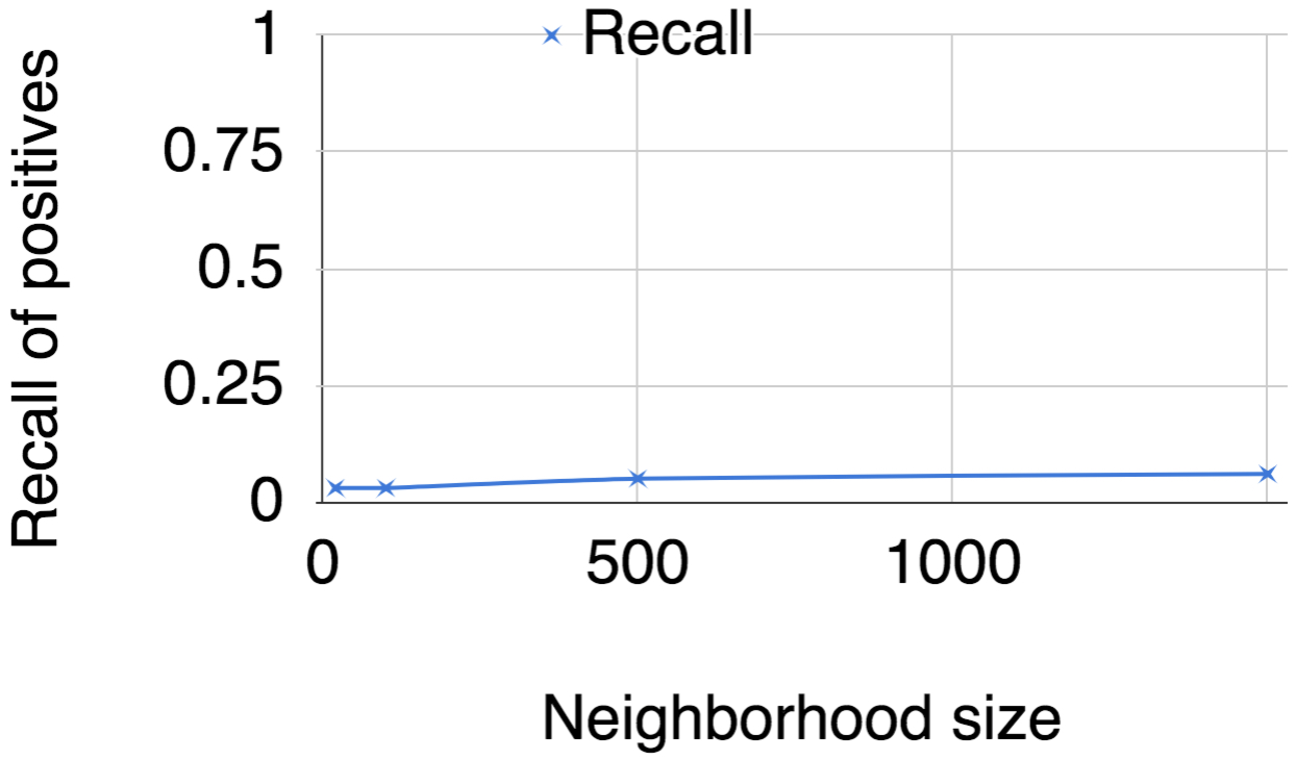
\includegraphics[width=.49\linewidth]{people_recall}
    }
    ~ 
    \subfloat[Mean negative distance as a function of neighborhood size\label{people_distance}]{%
        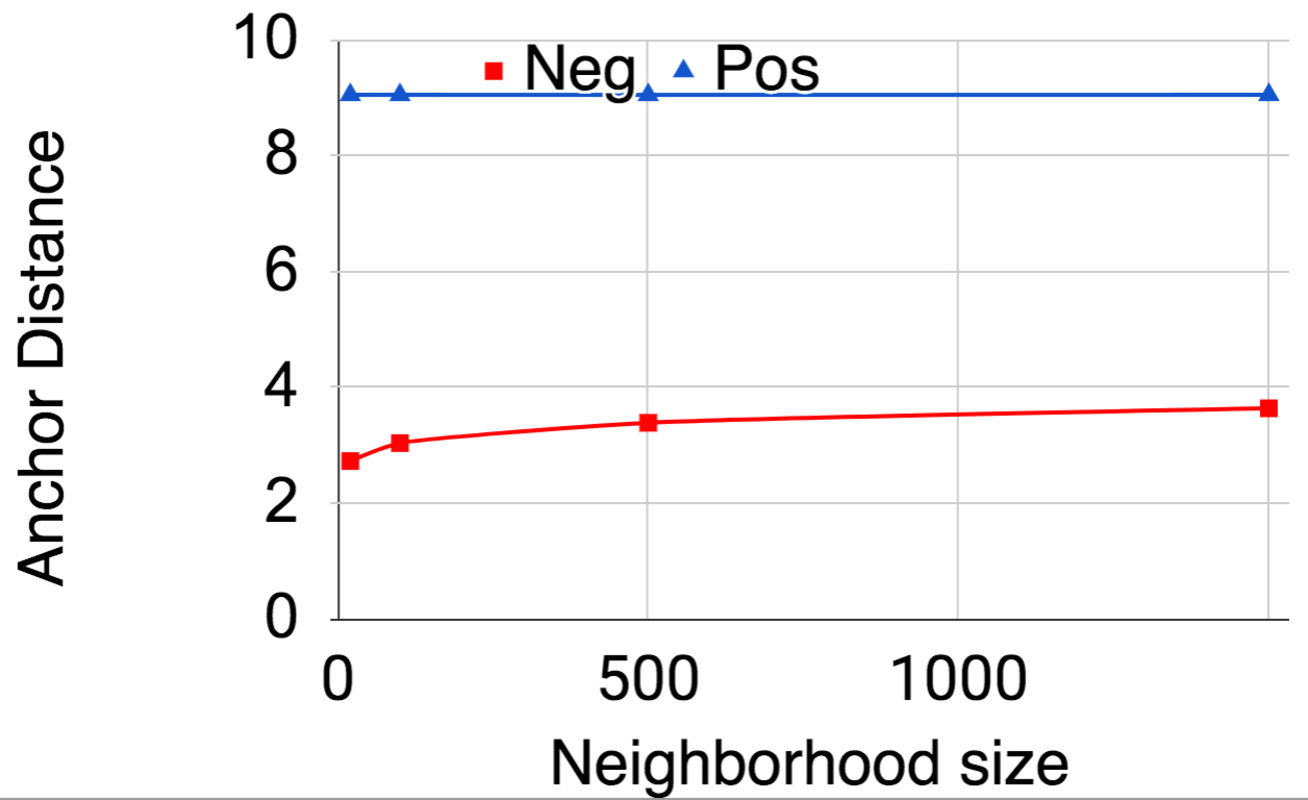
\includegraphics[width=.49\linewidth]{people_distances}
     }
    \label{people_distances}
    \caption{Characteristics of people data}
\label{people_characteristics}
\end{wrapfigure}

 As a baseline, we measured how the anchors, positives and negatives were laid out in vector space based on character embeddings alone.  This gives us a measure of how difficult the problem is for the neural network to learn.  We indexed all the vector embeddings (regardless of test or train) into a nearest neighbors algorithm using the Spotify ANNOY\footnote{\url{https://github.com/spotify/annoy}} implementation.  We then queried the index for the $k$ nearest neighbors of this set, varying $k$ so it was either 20, 100, 500, or 1500 neighbors.  Our primary interest was in recall rates of positives prior to any training, to establish the baseline prior to training.  We also measured the nature of hard negatives as we varied the neighborhoods; i.e., what is the mean distance of negatives from the anchor while we increased neighborhoods, compared to the positive distances.  Figure \ref{people_characteristics} shows the results for the people data.  First, recall rate of positives in the nearest neighbor set was very low at 3\%, and it increased only to 6\% at a neighborhood size of 1500.  The difficulty of the problem for reconciling people's names is further highlighted by the distance data.  The mean distance of positives from anchor was 9.05, with a standard deviation of 3.08.  The mean distances of negatives from anchor was 2.73, with a standard deviation of 0.99 for $k$ of 20.  However even for $k$ of 1500, the mean negative distance was 3.64, well below the mean positive distance of 9.05.  The company data show a similar trend, although companies seems to be an easier problem than reconciling people data, as shown in Figure \ref{company_characteristics}.  Recall rate for companies starts at 16\% for a neighborhood size of 20, and is up to 25\% for a neighborhood size of 1500.  Mean negative distance is at 3.05 compared to 4.64 at a neighborhood size of 20, with a standard deviation of 1.44.  At a neighborhood size of 1500, mean negative sizes are slightly higher at 3.86. 

\begin{wrapfigure}{r}{.65\textwidth}
   \subfloat[Recall rate as a function of neighborhood size\label{company_recall}]{%
        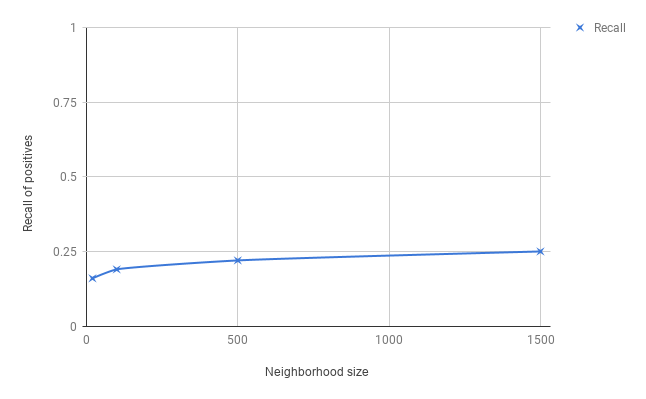
\includegraphics[width=.49\linewidth]{company_recall}
   }
   ~
   \subfloat[Mean negative distance from anchor as a function of neighborhood size \label{company_distance}]{%
        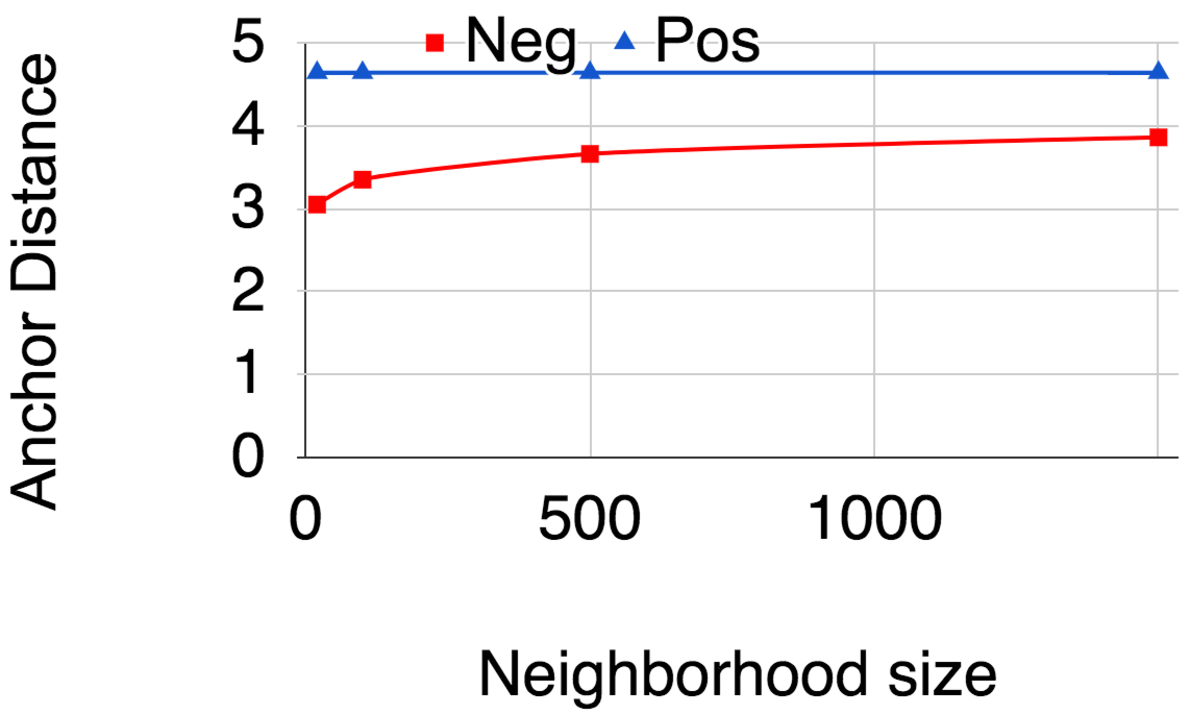
\includegraphics[width=.49\linewidth]{company_distances}
   }
    \label{company_distances}
    \caption{Characteristics of company data}
\label{company_characteristics}
\end{wrapfigure}
